% Preamble
\documentclass[12pt]{simple_doc}

% Packages
\usepackage{simple_note}
\usepackage{tkz-euclide}
\hypersetup{
    colorlinks=true,
    linkcolor=ctbPinkDark,
}
\usepackage{amsmath} % to remove equation numbers

% Document
\begin{document}
    \exerheader{Math}{Geometry}{\today}{ctbRedDark}

    \begin{cbstripe}{Problem}{ctbHoneyDark}{ctbHoneyLight}
        A point inside a square are connected to all side midpoints.
        Given the areas of 3 regions, find the area of the shaded. \medskip

        \centering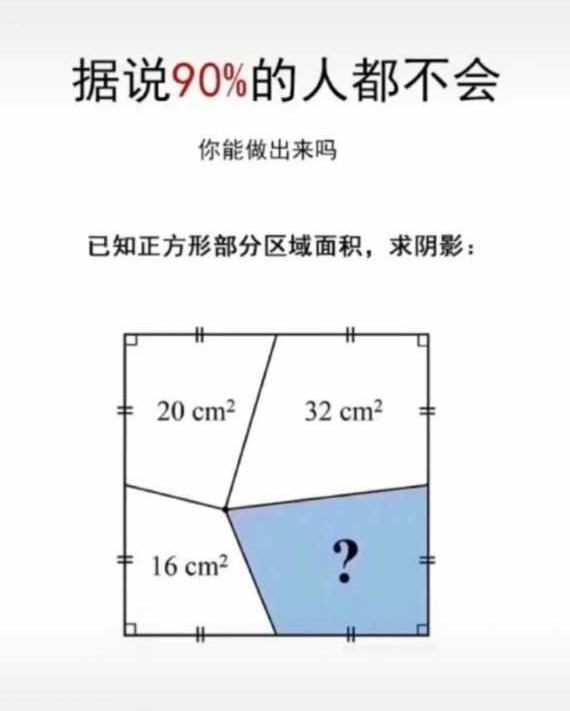
\includegraphics[scale=.3]{square_area}
    \end{cbstripe}

    The key to solve this problem is to divide non-triangle regions to triangle regions in order
    to see details of the given conditions. Once we do that, we can see the triangle areas are
    in pairs.

    \pgfmathsetmacro{\sqrtsix}{2.44949} % sqrt(6)
    \pgfmathsetmacro{\midpoint}{2 * \sqrtsix}
    \pgfmathsetmacro{\side}{4 * \sqrtsix}
    \pgfmathsetmacro{\pointy}{5.0 / 3 * \sqrtsix}

    \begin{center}
	\begin{tikzpicture} [scale=0.8]
        \tkzDefPoint (0, 0){A}
		\tkzDefPoint (\side, 0){B}
        \tkzDefPoint (\side, \side){C}
        \tkzDefPoint (0, \side){D}

        \tkzDefPoint (\sqrtsix, \pointy){P}
        \tkzDefPoint (\midpoint, 0){M1}
		\tkzDefPoint (\side, \midpoint){M2}
		\tkzDefPoint (\midpoint, \side){M3}
        \tkzDefPoint (0, \midpoint){M4}

        \fill[blue!5] (A) -- (P) -- (M1) --cycle; % fill in colors
        \fill[blue!5] (A) -- (P) -- (M4) --cycle;
        \fill[cyan!5] (B) -- (P) -- (M1) --cycle;
        \fill[cyan!5] (B) -- (P) -- (M2) --cycle;
        \fill[orange!5] (C) -- (P) -- (M2) --cycle;
        \fill[orange!5] (C) -- (P) -- (M3) --cycle;
        \fill[red!5] (D) -- (P) -- (M3) --cycle;
        \fill[red!5] (D) -- (P) -- (M4) --cycle;

        \tkzDrawPolygon[thick](A,B,C, D); % draw square

        \draw [thick] (M1) -- (P); % P to all 4 mid points
        \draw [thick] (M2) -- (P);
        \draw [thick] (M3) -- (P);
        \draw [thick] (M4) -- (P);
        \tkzMarkSegment[color=blue,pos=0.5,mark=||](A, M1) % mark equal
        \tkzMarkSegment[color=blue,pos=0.5,mark=||](M1, B)
        \tkzMarkSegment[color=blue,pos=0.5,mark=||](B, M2)
        \tkzMarkSegment[color=blue,pos=0.5,mark=||](M2, C)
        \tkzMarkSegment[color=blue,pos=0.5,mark=||](C, M3)
        \tkzMarkSegment[color=blue,pos=0.5,mark=||](M3, D)
        \tkzMarkSegment[color=blue,pos=0.5,mark=||](D, M4)
        \tkzMarkSegment[color=blue,pos=0.5,mark=||](M4, A)

        \draw [dashed, thick] (A) -- (P); % P to all 4 mid points
        \draw [dashed, thick] (B) -- (P);
        \draw [dashed, thick] (C) -- (P);
        \draw [dashed, thick] (D) -- (P);

        \tkzLabelPoint[red,anchor=center](\sqrtsix, 1.7){$A$}
        \tkzLabelPoint[red,anchor=center](5.0, 1.7){$A$}
        \tkzLabelPoint[red,anchor=center](1.0, 3.4){$B$}
        \tkzLabelPoint[red,anchor=center](1.0, 5.6){$B$}
        \tkzLabelPoint[red,anchor=center](2.45, 7.5){$C$}
        \tkzLabelPoint[red,anchor=center](5.1, 7.5){$C$}
        \tkzLabelPoint[red,anchor=center](6.0, 5.5){$D$}
        \tkzLabelPoint[red,anchor=center](6.0, 3.4){$D$}

	\end{tikzpicture}
	\end{center}

    Notice that sum of opposite regions have same triangle areas, $ A + B + C + D$
    \begin{equation*}
		\begin{aligned}
            A + D (right lower) &= A + B (lower\ left) + C + D (upper\ right) - (B + C) (upper\ left)\\
                                &= 16 + 32 - 20\\
                                &= 28
        \end{aligned}
	\end{equation*}

    Now to go one step further, we want to know the length of the square and the coordinates of the
    internal point(P). Assume square side has length $2a$ and P's coordinate is $(x, y)$. From the given
    areas of the 3 regions, we derive the following equations

    \begin{equation*} % star removes equation number
        \frac{1}{2} xa + \frac{1}{2} ya = 16
    \end{equation*}
    \begin{equation*}
        \frac{1}{2} xa + \frac{1}{2} (2a-y)a = 20
    \end{equation*}
    \begin{equation*}
        \frac{1}{2} (2a-y)a + \frac{1}{2} (2a-x)a = 32
    \end{equation*}

    The solution is
    \begin{equation*}
        a = 2\sqrt{6},\ x = \sqrt{6},\ and\ y = \frac{5}{3}\sqrt{6}
    \end{equation*}

    So $x$ is half of $a$, a quarter of the square side length. $y$ is near side midpoint.
    These are used to draw the picture.

    \href{https://mindyourdecisions.com/blog/2018/07/26/solve-for-the-shaded-area-you-should-be-able-to-solve-this/}{Here}
    has the same solution and more similar problems.
\end{document}
